\chapter{Stochastique: prise en compte de la variabilité}\label{Ch-stocha}
\begin{abstract}
Certains diront que c'est enfin dans ce chapitre que nous traitons de la réalité physique... c'est un point de vue.
En effet, rien n'est jamais connu de manière parfaite.

L'aléa traduit aussi bien l'impossibilité d'une description déterministe exhaustive que l'irrégularité de tout phénomène observé.
Les modèles déterministes ne sont finalement que des approximations des problèmes physiques correspondants, tout comme les modèles linéaires ne sont que des approximations de comportements réels non-linéaires par nature.

Nous nous restreindrons dans le nombre de formulations afin de ne présenter que ce qui nous semble aujourd'hui le plus pertinent.
\end{abstract}

\section{Introduction}

Dans la manière traditionnelle, encore appelée approche déterministe, la conception des structures repose sur des paramètres tels que les dimensions, la résistance des matériaux et le chargement, tous caractérisés par une valeur constante, i.e. leur moyenne. Sur la base de ces constantes on utilise un modèle mathématique du comportement pour déterminer si la structure est sûre ou non. Afin d'améliorer encore la sécurité, les variables structurelles sont alors remplacées par leur pire cas. Cette philosophie de conception se révèle trop coûteuse d'un point de vue économique car on se place dans le cas où toutes les paramètres sont à leur pire valeur en même temps.

Il est bien connu que, par exemple, la résistance varie d'un élément structurel à l'autre, de sorte que cette résistance ne peut être décrite par une unique valeur. De plus, il est parfois nécessaire de prendre en compte des variations temporelles. Ces mêmes variations existent également pour les dimensions et le chargement. Cela est particulièrement vrai pour les chargements naturels comme la houle, le vent et les séismes, qu'il est difficile de prendre en compte de manière déterministe. Il faut en outre garder en tête qu'une certaine incertitude existe également dans le choix des modèles mathématiques utilisés pour l'analyse de la structure.

Le but d'utiliser une approche probabiliste plutôt qu'une simple approche déterministe est d'essayer de prendre en compte les incertitudes mentionnées ci-dessus afin de réaliser une analyse plus réaliste de la sûreté de la structure.

\medskip
Dans ce chapitre, nous considérerons le problème de formulation classique suivant:
\begin{equation}\label{Eq-Sto1}
au=f
\end{equation}
Jusqu'à présent, nous nous sommes contenté du cas où~$a$ est un opérateur déterministe,~$f$ l'excitation déterministe et~$u$ la réponse déterministe.
Nous allons dans ce chapitre nous intéresser au cas où~$f$ est une excitation aléatoire et~$a$ un opérateur éventuellement aléatoire. Il s'en suit que la réponse du système~$u$ est elle-aussi aléatoire.

\medskip
La manipulation d'équations stochastiques introduit deux difficultés:
\begin{itemize}
   \item premièrement, les propriétés aléatoires du système doivent être modélisées «correctement» comme variables ou processus aléatoires, avec une distribution de probabilité réaliste;
   \item deuxièmement, il faut être capable de résoudre le système différentiel ainsi obtenu, et la réponse obtenue doit pouvoir être décrite par ses moments statistiques.
\end{itemize}

\medskip
Enfin, la relation entre éléments finis et probabilité recouvre deux aspects:
\begin{itemize}
   \item d'une part le calcul des moments statistiques de la réponse autour de sa moyenne (essentiellement l'écart-type);
   \item d'autre part les méthodes de fiabilité, par lesquelles on cherche à calculer une probabilité de défaillance associée à un critère dont les arguments dépendent du résultat d'un calcul par éléments finis.
\end{itemize}
%Nous présenterons ces deux approches dans ce chapitre.

\begin{histoire}
Les séries de fonctions, apparues à la fin du \textsc{xvii}\fup{e} siècle, et particulièrement les séries de Taylor\index[aut]{Taylor (Brook), 1685-1731, Anglais} (voir historique du paragraphe~\ref{Sec-Taylor}), sont aujourd'hui un outil indispensable, permettant notamment d'approcher une fonction de manière facilement exploitable.
C'est pourquoi la manière la plus naturelle d'appréhender le traitement de l'équation~(\ref{Eq-Sto1}) a été de procéder à un développement en série.

\sbox{\MaBoiteAvecPhotos}{\setlength{\tabcolsep}{0pt}\scriptsize%
\begin{tabular}{ccc}%
\includegraphics[height=\the\HauteurDesPhotos]{Kolmogorov2}&%
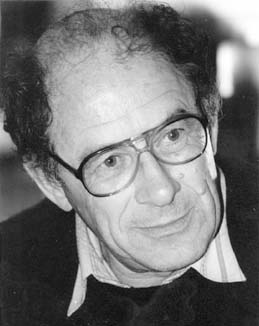
\includegraphics[height=\the\HauteurDesPhotos]{ArnoldV}&%
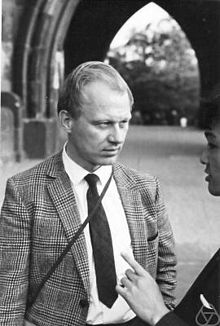
\includegraphics[height=\the\HauteurDesPhotos]{Moser}\\%
Kolmogorov&Arnold&Moser%
\end{tabular}}
\medskip
\ImageADroite{%
Dès le début du \textsc{xviii}\fup{e} siècle, la \textcolorblue{théorie des perturbations} a été utilisée par les astronomes pour les besoins de la mécanique céleste: en effet, les équations différentielles décrivant un système de~$n$ corps en interaction gravitationnelle n'a pas de solution exacte générale pour~$n\ge3$. Cet aspect de la théorie des perturbations a été synthétisé à la fin du \textsc{xix}\fup{e} siècle dans les ouvrages classiques de Laplace,\index[aut]{Lagrange (Joseph Louis, comte de -), 1736-1813, Italien} Tisserand\index[aut]{Tisserand (François Félix), 1845-1896, Français} et Poincaré,\index[aut]{Poincaré (Henri), 1854-1912, Français} avant de connaître de nouveaux développements dans la seconde moitié du \textsc{xx}\fup{e} siècle avec l'avènement en 1954 de la «théorie KAM» ( théorème de mécanique classique i.e. non relativiste et non quantique, mettant en défaut l'hypothèse ergodique de Boltzmann),\index[aut]{Boltzmann (Ludwig), 1944-1906, Autrichien} du nom de ses trois concepteurs: Kolmogorov,\index[aut]{Kolmogorov (Andreï Nikolaïevitch), 1903-1987, Russe} Arnold\index[aut]{Arnold (Vladimir Igorevitch), 1937-2010, Russe} et Moser.\index[aut]{Moser (Jürgen Kurt), 1928-1999, Allemand} La méthode a par ailleurs été abondamment utilisée au \textsc{xx}\fup{e} siècle pour les besoins de la physique quantique, d'abord en mécanique quantique non relativiste, puis en théorie quantique des champs perturbative.}

\medskip
C'est encore cette même méthode de perturbation qui est la plus ancienne et la plus utilisée en ingénierie pour analyser les systèmes aléatoires (pas seulement aléatoires, voir la présentation de la méthode de réanalyse au paragraphe~\ref{Sec-PInv} qui est une méthode de perturbation).
Bien que les méthodes mathématiques sous-jacentes soient très simples, cela ne signifie nullement que leur validité aille de soi: on fait un développement de Taylor\index[aut]{Taylor (Brook), 1685-1731, Anglais} de chaque quantité aléatoire autour de sa moyenne, les termes causant l'instabilité de la solution approchée étant d'ordres supérieurs. Toutefois, dans la pratique, il n'est pas possible d'aller au delà de l'ordre un ou deux. Cela réduit la portée des applications de la méthode aux cas des \textcolorgreen{petits aléas, i.e. de petites fluctuations autour d'une valeur moyenne}. Sans efforts inconsidérés, \textcolorred{ces méthodes ne fournissent pas de statistiques d'ordres élevés.}

\medskip
Il a donc bien évidemment été essayé d'améliorer cette méthode afin d'obtenir des statistiques d'ordres plus élevés. Une méthode, peu connue et peu utilisée, pour atteindre ce but est la \textcolorblue{hierarchy closure approximation}. Il s'agit d'exprimer les moments d'ordres élevés en fonctions de moments d'ordres moins élevés.
Si l'on considère que l'opérateur~$a$ de l'équation~(\ref{Eq-Sto1}) peut être décomposé en une partie déterministe~$\overline{a}$ et une partie aléatoire~$\widetilde{a}$, cette équation se met sous la forme:
\begin{equation}
(\overline{a}+\widetilde{a})u=f
\end{equation}
qui se résout en:
\begin{equation}
u=\overline{a}^{-1}f-\overline{a}^{-1}\widetilde{a}u
\end{equation}
En appliquant à cette dernière équation l'opérateur~$\widetilde{a}$, puis en réinjectant le résultat dans l'équation précédente, il vient:
\begin{equation}
u=\overline{a}^{-1}f-\overline{a}^{-1}\widetilde{a}\overline{a}^{-1}f+\overline{a}^{-1}\widetilde{a}\overline{a}^{-1}\widetilde{a}u
\end{equation}
et on peut poursuivre ainsi, si on le souhaite. Cela ne peut néanmoins être fait que si:
\begin{equation}\label{Eq-Unco}
\E{\PP{\overline{a}^{-1}\widetilde{a}}^nu} = \E{\PP{\overline{a}^{-1}\widetilde{a}}^n}\E{u}
\end{equation}
où~$\E{.}$ est la moyenne (espérance mathématique).

\textcolorgreen{Le découplage effectué par l'équation~(\ref{Eq-Unco}) n'a pas de base rigoureuse et est souvent justifié intuitivement par un argument d'indépendance locale.} \colorred On aboutit de toutes façons à une formulation très complexes \colorred pour les moments d'ordres élevés,\colorblack de sorte que cette méthode n'est utilisée en pratique elle aussi que pour le cas des petites fluctuations.
\end{histoire}

\medskip
\section{Représentation des processus stochastiques}

Nous allons reprendre et compléter ce qui a été présenté au paragraphe \ref{Sec-Mesure}.
Nous avons donc déjà exposé qu'une probabilité est une mesure particulière.
Reprenons cela avec un vocabulaire probabiliste.

\medskip
\subsection{Variable aléatoire}

On appelle \textcolorblue{épreuve} l'observation d'un phénomène aléatoire.
Toutes les \textcolorblue{réalisations} possibles d'une épreuve forment l'ensemble de tous les résultats d'une expérience aléatoire, qui sera noté~$\Theta$.
Un \textcolorblue{événement}~$E$ est un sous-ensemble de~$\Theta$ contenant les réalisations~$\theta\in\Theta$.
La \textcolorblue{mesure} de l'occurrence de~$E$ est une mesure de probabilité notée~$P$.
L'ensemble de tous les événements possibles ayant une probabilité ainsi définie est appelé une~$\sigma$-algèbre associée à~$\Theta$, et est notée~$\mathcal{F}$.
L'espace de probabilité construit grâce à ces notions est noté~$(\Theta,\mathcal{F},P)$.
En d'autres termes, pour reprendre la partie I, l'espace de probabilité~$(\Theta,\mathcal{F},P)$ est construit sur la tribu~$\mathcal{F}$ et avec la mesure~$P$.

\medskip
Une \textcolorblue{variable aléatoire} réelle~$X$ est une fonction~$X : (\Theta,\mathcal{F},P) \rightarrow \RR$.
Pour les variables aléatoires continues, la \textcolorblue{densité de probabilité} est notée~$f_X(x)$ et la \textcolorblue{fonction de répartition} est notée~$F_X(x)$.
Un \textcolorblue{vecteur aléatoire} est un vecteur dont les composantes sont des variables aléatoires.

\medskip
\begin{definition}[Moments d'une variables aléatoire]
Les \textcolorblue{moments d'ordre~$n$} d'une variable aléatoire~$X$, s'ils existent, sont définis par:
\begin{equation}
\E{X^n} = \dint_{-\infty}^\infty x^nf_X(x)dx
\end{equation}
et les moments centrés réduits, s'ils existent, sont:
\begin{align}
\text{moyenne: } & \mu = \LLP{X} = \E{X} = \dint_{-\infty}^\infty xf_X(x) \dd x  \\
\text{variance: } & \sigma^2 = \E{(X-\mu)^2} = \dint_{-\infty}^\infty (x-\mu)^2f_X \dd x \\
\text{coefficient d'asymétrie (skewness): } & \delta = \dfrac{\E{(X-\mu)^3}}{\sigma^3} \\
\text{coefficient d'aplatissement (kurtosis): } & \kappa = \dfrac{\E{(X-\mu)^4}}{\sigma^4}
\end{align}
\end{definition}
\textcolorgris{La variance est égale au carré de l'écart-type.}

\medskip
\subsection{Espace de probabilité}

Soient maintenant deux variables aléatoires~$X$ et~$Y$.
La \textcolorblue{covariance} de ces deux variables est:
\begin{equation}
\cov{X,Y}=\E{(X-\mu_X)(Y-\mu_Y)}=\dint_{-\infty}^\infty\dint_{-\infty}^\infty(x-\mu_X)(y-\mu_Y)f_{X,Y}(x,y)\dd x\dd y
\end{equation}
où~$f_{X,Y}$ est leur \textcolorblue{densité de probabilité conjointe}.

\medskip
\begin{definition}
L'\textcolorblue{espace vectoriel des variables aléatoires réelles d'écart-type fini} (moment d'ordre 2), noté~$L^2(\Theta,\mathcal{F},P)$, est un espace de Hilbert.

\textcolorgris{Le produit scalaire sur cet espace de Hilbert est défini comme:
$(X,Y)=\int xy\dd P$
où~$\dd P$ est la mesure de probabilité conjointe, ce qui équivaut à~$(X,Y)=\int xyf_{X,Y}\dd x\dd y$.}
Avec ce qui précède, le produit scalaire est donc finalement défini par:
\begin{equation}\label{Eq_StoPS}
(X,Y)=\E{XY}
\end{equation}
et la norme associée est:
\begin{equation}
\|X\|=\sqrt{\E{X^2}}
\end{equation}
\end{definition}

\begin{theoreme}
Les polynômes d'Hermite\index{polynôme!d'Hermite} sous leur forme probabiliste,~$H_n$, présentés au paragraphe \ref{Sec-PolHermite}, forment une base de l'espace~$L^2(\Theta,\mathcal{F},P)$.
\end{theoreme}

On rappelle également qu'une variable aléatoire gaussienne centrée réduite (i.e. de moyenne nulle, écart-type égal à 1) a une densité de probabilité~$\varphi$ et une fonction de répartition~$\Phi$ définies par:
\begin{equation}
\varphi(x) =\frac{\mathrm{e}^{-x^2/2}}{\sqrt{2\pi}} \quad \text{ et } \quad
\Phi(x) = \dfrac1{\sqrt{2\pi}}\dint_{-\infty}^x \mathrm{e}^{-t^2/2} \dd t
\end{equation}
\textcolorblue{Dans la suite du chapitre, nous noterons~$\xi$ une telle variable aléatoire gaussienne centrée réduite.}

\medskip
Nous présentons quelques propriétés des polynômes d'Hermite,\index{polynôme!d'Hermite} à commencer par la relation d'orthogonalité:\index{polynôme!orthogonalité}
\begin{equation}
  \int_{-\infty}^{+\infty} H_n(x)H_m(x)\varphi(x)\dd x=n!\delta_{nm}
\end{equation}
où~$\delta_{nm}$ est le symbole de Kronecker.
\begin{equation}
\dfrac{\dd H_n(x)}{\dd x} = nH_{n-1}(x)
\end{equation}
\begin{equation}
H_i(x)H_j(x)=\dsum_{k=|i-j|}^{i+j} C_{ijk}H_k(x)
\end{equation}
avec:
\begin{equation}
\left\{\begin{array}{rll}
C_{ijk} &=0& \text{ si } \frac{i+j+k}2\not\in\NN\\
C_{ijk} &=\dfrac{i!j!}{\PP{\frac{i+j-k}2}!\PP{\frac{i+k-j}2}!\PP{\frac{j+k-i}2}!}& \text{ sinon }
\end{array}
\right.
\end{equation}


\medskip
\subsection{Processus ou champ aléatoire}

Nous venons de présenter les variables aléatoires.
Or, ce qui nous intéresse, est de prendre en compte la variation d'une propriété (par exemple le module d'Young du matériau) continûment sur notre domaine~$\Omega$.

\begin{definition}[Champ aléatoire ou processus stochastique]
Un \textcolorblue{champ aléatoire scalaire}~$w(x,\theta)$ peut être défini comme un ensemble de variables aléatoires indexées par un paramètre continu~$x\in\Omega$.
\textcolorgris{le paramètre~$x$ n'est pas forcément continu, il peut être discret. Nous nous intéressons ici au cas d'un processus continu.}
Ainsi un \textcolorblue{processus stochastique}~$w(x,\theta)$ définit une fonction de deux variables~$x$ et~$\theta$ et représente:
\begin{itemize}
   \item~$x$ et~$\theta$ variables: une famille de fonctions;
   \item~$x$ variable et~$\theta$ fixé: une fonction de~$x$, i.e. une réalisation du champ aléatoire (i.e. une fonction de~$\RR^d$ dans~$\RR$, où notre domaine~$\Omega$ est un ouvert de~$\RR^d$);
   \item~$x$ fixé et~$\theta$ variable: une variable aléatoire;
   \item~$x$ et~$\theta$ fixés: un nombre.
\end{itemize}
\end{definition}
Un champ aléatoire est dit:
\begin{itemize}
   \item \textcolorblue{vectoriel} si la quantité~$w(x,\theta)$ attachée au point~$x$ est un vecteur aléatoire.
   \item \textcolorblue{unidimensionnel} si~$d=1$ et \textcolorblue{multidimensionnel} sinon (cas qui nous intéresse).
   \item \textcolorblue{gaussien} si tout vecteur~$\{w(x_1), ..., w(x_n)\}$ est un vecteur gaussien. Il est alors complètement défini par sa moyenne, sa variance et sa fonction d'autocovariance définie par:
   \begin{equation}
       C(x,x')=\cov{w(x),w(x')}
   \end{equation}
   \item \textcolorblue{stationnaire (au sens faible)} si sa moyenne et sa variance sont constantes et si sa fonction d'autocorrélation~$\rho$ ne dépend que de la différence~$(x-x')$. La fonction d'autocorrélation est définie par:
   \begin{equation}
      \rho(x,x')=\dfrac{C(x,x')}{\sigma(x)\sigma(x')}
   \end{equation}
\end{itemize}

\medskip
\subsection{Discrétisation de champs aléatoires}

Maintenant que nous avons défini ce qu'est un processus stochastique~$w(x,\theta)$, il nous faut le discrétiser.
On se propose donc d'approcher~$w(x,\theta)$ par~$w_h(x,\chi)$, où~$\chi$ est un vecteur aléatoire constitué de~$n$ variables aléatoires~$\xi_i$, i.e. sous la forme:
\begin{equation}
w(x,\theta)\approx w_h(x,\chi)
\end{equation}
Plusieurs méthodes sont possibles:
\begin{description}
   \item[\textcolorblue{discrétisation par valeurs moyennes:}] les~$\xi_i$ sont des intégrales pondérées de~$w(x,\theta)$ sur un domaine~$\Omega_i$, et dans le cas des éléments finis, sur chaque élément. Cette méthode a pour conséquence de lisser le processus stochastique;
   \item[\textcolorblue{discrétisation par valeurs ponctuelles:}] les~$\xi_i$ sont sélectionnées parmi les valeurs de~$w(x,\theta)$ en certains points~$x$. Cette méthode de collocation a pour conséquence de générer des irrégularités additionnelles;
   \item[\textcolorblue{développement en séries:}] le champ est représenté par une série de variables aléatoires et de fonctions spatiales déterministes. C'est uniquement ce type de méthode que nous allons présenter.
\end{description}


\medskip\ifVersionDuDocEstVincent\else\newpage\fi
\subsection{Développement en série de Karhunen-Loève}\index{série de Karhunen-Loève}

\begin{histoire}
Nous avons déjà mentionné dans ce chapitre que la méthode de perturbation, basée sur un développement en série de Taylor,\index[aut]{Taylor (Brook), 1685-1731, Anglais} avait des limitations.
%\medskip
\sbox{\MaBoiteAvecPhotos}{\setlength{\tabcolsep}{0pt}\scriptsize%
\begin{tabular}{cccc}%
\includegraphics[height=\the\HauteurDesPhotos]{Karhunen}&%
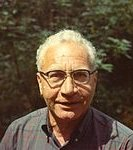
\includegraphics[height=\the\HauteurDesPhotos]{Loeve}&%
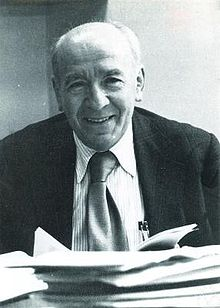
\includegraphics[height=\the\HauteurDesPhotos]{Kac}&
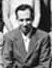
\includegraphics[height=\the\HauteurDesPhotos]{Siegert}\\
Karhunen&Loève&Kac&Siegert%
\end{tabular}}
\medskip
\ImageADroite{%
Toutefois, le recourt à un développement en série reste une idée intéressante... reste à trouver comment procéder.\\ \indent
Pour améliorer le développement en série d'un champ aléatoire, on peut penser à utiliser un développement à la Fourier: scinder la dépendance des variables~$x$ et~$\theta$, et utiliser une base de fonctions orthogonales.
Ainsi cherche-ton a écrire le processus stochastique~$w(x,\theta)$ sous la forme:}
\begin{equation}
w(x,\theta)=\dsum_{i=0}^\infty \alpha_i\xi_i(\theta)f_i(x)
\end{equation}
où les~$\alpha_i$ sont des constantes à déterminer, les~$\xi_i$ des variables aléatoires et les~$f_i$ des fonctions déterministes orthogonales entre elles.
C'est exactement ce que propose le développement de Karhunen-Loève,\index[aut]{Karhunen (Kari), 1915-1992, Finlandais}\index[aut]{Loève (Michel), 1907-1979, Français} obtenu indépendamment par Karhunen en 1947, Loève\index[aut]{Loève (Michel), 1907-1979, Français} en 1948, mais également en 1947 par Kac\index[aut]{Kac (Mark ou Marek), 1914-1984, Américain} et son ami Siegert\index[aut]{Siegert (Arnold John Frederick), 1911-1995, Américain} du Radiation Laboratory.
\end{histoire}

La méthode de Karhunen-Loève\index[aut]{Karhunen (Kari), 1915-1992, Finlandais}\index[aut]{Loève (Michel), 1907-1979, Français} se propose elle-aussi de décomposer le champ aléatoire~$w(x,\theta)$ en une partie déterministe (sa moyenne~$\mu(x)$) et une partie aléatoire.
Cette fois, la partie aléatoire sera décomposée sur la base des valeurs propres~$\lambda_i$ et des fonctions propres~$\varphi_i(x)$ de la fonction d'autocovariance
\begin{equation}
C_{ww}(x,x')=\sigma(x)\sigma(x')\rho(x,x')
\end{equation}
Il faut donc résoudre le problème aux valeurs propres suivant:
\begin{equation}
\dint_\Omega C_{ww}(x,x')\varphi(x')\dd \Omega = \lambda_i\varphi_i(x), \quad \forall i\ge 1
\end{equation}
qui est une équation intégrale de Fredholm\index[aut]{Fredholm (Ivar), 1866-1927, Suédois} de deuxième espèce.
Le noyau~$C_{ww}(.,.)$ étant une fonction d'autocovariance, il est borné, symétrique et défini positif (Loève,\index[aut]{Loève (Michel), 1907-1979, Français} 1977). l'ensemble des~$\{\varphi_i\}$ forme une base complète orthogonale de l'espace des fonctions~$L^2(\Omega)$. Les valeurs propres sont réelles, positives et en nombre fini.

\medskip
Chaque réalisation de~$w$ peut donc être développée sur cette base sous la forme:
\begin{equation}\label{Eq-KL}
w(x,\theta) = \mu(x) + \dsum_{i=1}^\infty \sqrt{\lambda_i}\xi_i(\theta)\varphi_i(x)
\end{equation}
où les~$\xi_i$ sont les coordonnées de la réalisation du champ aléatoire par rapport à l'ensemble des fonctions déterministes~$\varphi_i$.

On montre aisément que~$\E{\xi_m\xi_n}=\delta_{mn}$ et~$\E{\xi_n}=0$. La famille~$\{\xi_i\}_{i\ge1}$ forme un ensemble orthonormal de variables aléatoires.

\medskip
Comme il ne peut y avoir de valeurs propres multiples (sauf 0), il est possible de les classer en une suite décroissante. En tronquant la somme de l'équation~(\ref{Eq-KL}) à l'ordre~$M$ (i.e. en ne retenant que les~$M$ plus grands valeurs propres), on obtient l'approximation de Karhunen-Loève\index[aut]{Karhunen (Kari), 1915-1992, Finlandais}\index[aut]{Loève (Michel), 1907-1979, Français}\index{série de Karhunen-Loève} du champ aléatoire:
\begin{equation}\label{Eq-KL}
w_h(x,\theta) = \mu(x) + \dsum_{i=1}^M \sqrt{\lambda_i}\xi_i(\theta)\varphi_i(x)
\end{equation}
\medskipvm
Comme les fonction propres sont orthonormales, on obtient une expression de chacune des variables aléatoires~$\xi_i$ apparaissant dans la série de Karhunen-Loève:\index[aut]{Karhunen (Kari), 1915-1992, Finlandais}\index[aut]{Loève (Michel), 1907-1979, Français}\index{série de Karhunen-Loève}
\begin{equation}
\xi_i(\theta)=\dfrac1{\sqrt{\lambda_i}}\dint_\Omega \PP{w(x,\theta)-\mu(x)}\varphi_i(x)\dd\Omega
\end{equation}
Cette dernière équation nous dit également que lorsque~$w$ est un champ gaussien, alors chaque variable aléatoire~$\xi_i$ est également gaussienne.
Les~$\{\xi_i\}_{i\ge1}$ forment un ensemble de variables aléatoires gaussiennes centrées réduites indépendantes.


\medskip
\subsection{Chaos polynomial}\index{chaos polynomial}

\begin{histoire}
La théorie des fonctionnelles non-linéaires a été développée par Volterra\index[aut]{Volterra (Vito), 1860-1940, Italien} dès 1913.
Il généralisa le développement des fonctions en série de Taylor au cas des fonctionnelles.
\sbox{\MaBoiteAvecPhotos}{\setlength{\tabcolsep}{0pt}\scriptsize%
\begin{tabular}{cccc}%
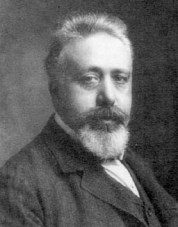
\includegraphics[height=\the\HauteurDesPhotos]{Volterra}&%
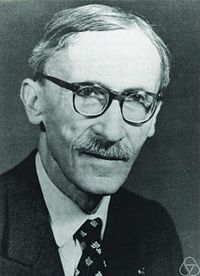
\includegraphics[height=\the\HauteurDesPhotos]{Levy}&%
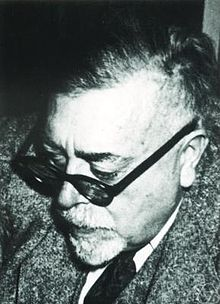
\includegraphics[height=\the\HauteurDesPhotos]{Wiener}&%
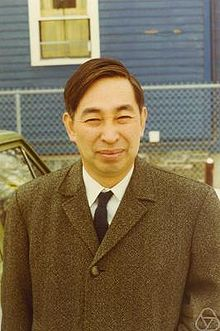
\includegraphics[height=\the\HauteurDesPhotos]{Ito}\\%
Volterra&Lévy&Wiener&It$\overline{\text{o}}$%
\end{tabular}}
\medskip
\ImageADroite{%
Wiener\index[aut]{Wiener (Norbert), 1894-1964, Américain} s'intéressa au problème par ses contact avec Paul Lévy\index[aut]{Lévy (Paul Pierre), 1886-1971, Français}, élève de Volterra.
C'est lui qui appliqua les idées de Volterra pour la première fois à l'analyse stochastique. Il appliqua sa théorie du mouvement brownien à l'intégration des fonctionnelles de Volterra et développa ce que l'on appelle désormais le chaos homogène.\\ \indent
Poursuivant les travaux de Wiener, Cameron\index[aut]{Cameron (Robert Horton), 1908-1989, Américain} et Martin\index[aut]{Martin (William T.), 1911-2004, Américain} en 1947 proposèrent un développement de type Fourier pour les fonctionnelles non-linéaires: le développement de Fourier-Hermite.\index[aut]{Fourier (Jean Baptiste Joseph), 1768-1830, Français}\index[aut]{Hermite (Charles), 1822-1901, Français}
C'est à nouveau Wiener qui, à partir de ses travaux de 1923 sur les espaces différentiels et de 1938 sur les chaos homogène, appliqua le développement de Fourier-Hermite en 1958 aux problèmes impliquant des phénomènes aléatoires. Il en résultera le développement de Wiener-Hermite, qui a été appliqué depuis à une grande variété de problèmes.\\ \indent
Le chaos homogène de Wiener a ensuite été raffiné par It$\overline{\text{o}}$\index[aut]{It$\overline{\text{o}}$ (Kiyoshi), 1915-2008, Japonais} en 1951 pour obtenir ce que l'on appelle maintenant l'intégrale multiple de Wiener.}
\end{histoire}

\medskip
L'utilisation du développement de Karhunen-Loève\index[aut]{Karhunen (Kari), 1915-1992, Finlandais}\index[aut]{Loève (Michel), 1907-1979, Français}\index{série de Karhunen-Loève} nécessite de connaître la fonction de covariance du processus à développer.
Or, si l'on souhaite appliquer un tel développement aux coefficients aléatoires de l'opérateur dans l'équation~(\ref{Eq-Sto1})... et bien justement on ne connaît pas la fonction de covariance ni par conséquent ses fonctions propres.
Il est nécessaire de trouver un autre développement qui contourne le problème.

\medskip
Le chaos polynomial est une forme particulière du chaos homogène. Il est défini comme suit.

\begin{definition}[Chaos polynomial]\index{chaos polynomial}
Le \textcolorblue{chaos polynomial de dimension~$M$ et d'ordre~$p$} est défini comme l'ensemble des polynômes d'Hermite\index{polynôme!d'Hermite} multidimensionnels en les~$M$ variables aléatoires gaussiennes centrées réduites~$\xi_1$, ...,~$\xi_M$ de degré inférieur ou égale à~$p$.

Chacun de ces polynômes est complètement défini par une liste de~$M$ entiers positifs ou nuls~$\alpha_1$, ...,~$\alpha_M$ comme suit à partir des polynômes d'Hermite~$H_n$:
\begin{equation}
\Psi_\alpha = \prod_{i=1}^M H_{\alpha_i}(\xi_i)
\end{equation}
où~$\alpha$ est la liste considérée.
\end{definition}

\textcolorgris{L'ensemble des chaos polynomiaux est un sous-espace linéaire de l'espace des fonctions~$L^2$ de variables aléatoires~$\Theta$ défini plus haut, et est un anneau pour la multiplication fonctionnelle.}

\medskip
Déterminons la dimension de la base du chaos polynomial de dimension~$M$ et d'ordre~$p$:
\begin{demonstration}\footnotesize\colorgris
(On pourrait aboutir au résultat plus directement, mais nous en profitons pour parler des polynômes homogènes).
Considérons l'anneau des polynômes en~$M$ indéterminées~$\RR[X_1, ..., X_M]$.
Un polynôme homogène, ou forme algébrique, est un polynôme en plusieurs indéterminées dont tous les monômes non nuls sont de même degré total.
L'ensemble des polynômes homogènes de degré~$p$ dans~$\RR[X_1, ..., X_M]$ forme un~$\RR$-espace vectoriel.
%(le polynôme nul est homogène de degré~$p$, pour tout entier~$p$; c'est le seul polynôme homogène dont le degré n'est donc pas défini).
Sa base canonique est l'ensemble des monômes~$X_1^{\alpha_1}X_2^{\alpha_2}...X_M^{\alpha_M} \text{ où } \alpha_1+\alpha_2+...+\alpha_M=p$.
Sa dimension est donc le nombre de~$p$-combinaisons avec répétition de l'ensemble~$\{1, 2, ..., M\}$, i.e.~$\Gamma_M^p={M+p-1\choose p}$.
La dimension de cette base vaut~$\sum_{i=0}^p \Gamma_M^p$, avec~$\Gamma_M^0=1$.\normalsize\colorblack \\
Tous calculs faits, La dimension de la base du chaos polynomial de dimension~$M$ et d'ordre~$p$ est donc donnée par:
\begin{equation}
{M+p\choose p}
\end{equation}\footnotesize\colorgris~$\square$\colorblack
\end{demonstration}
Le tableau~\ref{Tab-NbChaos} donne le nombre de polynômes présents dans la base du chaos polynomial considéré en fonction du nombre~$M$ de variables aléatoires et du degré maximal~$p$ choisi.
\begin{table}[htb]
\begin{center}
\begin{tabular}{c|cccc}
& $p=1$ & $p=2$ & $p=3$ & $p=4$\\
\hline
$M=1$ &2&3&4&5\\
$M=2$ &3&6&10&15\\
$M=3$ &4&10&20&35\\
$M=4$ &5&15&35&70\\
$M=5$ &6&21&56&126\\
$M=6$ &7&28&84&210
\end{tabular}
\end{center}
\caption{Nombre de polynômes dans la base du chaos: $M$ est le nombre de variables aléatoires, et~$p$ le degré maximal}\label{Tab-NbChaos}
\end{table}


\medskip
\section{Éléments finis stochastiques}\index{élément fini!stochastique}

Nous rappelons l'équation~(\ref{Eq-Sto1}):
\begin{equation*}au=f \text{ que l'on peut écrire maintenant: } a(x,\theta) u(x,\theta) = f(x,\theta)\end{equation*}
où l'opérateur~$a$ est défini sur le produit d'un espace de Hilbert de type~$L^2$ (en fonction du problème) par l'espace de Hilbert~$L^2(\Theta,\mathcal{F},P)$.
C'est un opérateur différentiel dont les coefficients ont des fluctuations aléatoires dépendant d'une ou plusieurs variables.

\medskip
On fait l'\textcolorblue{hypothèse} que l'opérateur~$a$ est un opérateur différentiel dont les coefficients aléatoires sont contraints à être des \textcolorblue{processus stochastiques du second ordre}.
Cette hypothèse n'est pas sévère en fait, car la plupart des processus physiquement mesurables sont de ce type.
On pourra donc écrire chacun des coefficients~$a_i(x,\theta)$ de~$a$ comme la somme d'une composante déterministe~$\overline{a_i}(x)=\E{a_i(x,\theta)}$ et d'une composante aléatoire~$\widetilde{a_i}(x,\theta)$.
On obtiendra à nouveau un système sous la forme:
\begin{equation}\label{Eq-Sto2}
(\overline{a}(x)+\widetilde{a}(x,\theta))u(x,\theta)=f(x,\theta)
\end{equation}
qui se résout en:
\begin{equation}
u=g(\widetilde{a_i}(x,\theta),f(x,\theta))
\end{equation}
avec~$g$ une fonctionnelle non-linéaire.

\medskip
\subsection{Développement en séries de von Neumann}\index{série de von Neumann}

Notre problème consiste à résoudre l'équation~(\ref{Eq-Sto2}), i.e. à inverser l'opérateur.
Lorsque un opérateur est inversible, son inverse admet un développement en série convergeant.
La méthode de développement en séries de von Neumann\index[aut]{Neumann (John, von -), 1903-1957, Hongrois}\index{série de von Neumann} consiste a écrire la solution de l'équation~(\ref{Eq-Sto2}) sous la forme:
\begin{equation}\label{Eq-StoNeu}
u(\widetilde{a}(\theta),x)=\dsum_{i=0}^\infty (-1)^i \PP{\overline{a}^{-1}(x)\widetilde{a}(x,\theta)}^i f(x,\theta))
\end{equation}
qui ne converge que si:
\begin{equation}
\|\overline{a}^{-1}(x)\widetilde{a}(x,\theta)\| <1
\end{equation}
L'intérêt est que l'on ne doit inverser que~$\overline{a}^{-1}(x)$.
Toutefois, on ne sait pas calculer symboliquement les termes d'ordre supérieur à deux, et on se contente de simulations numériques au delà.
On peut faire les mêmes remarques que pour la méthode de perturbation et il est difficile d'obtenir les moments d'ordre supérieur à deux, surtout si l'on considère la valeur moyenne du processus sur chaque élément, comme nous allons l'illustrer immédiatement en mécanique.

\medskip
\subsection{Un exemple en statique linéaire}

Considérons le cas de la statique linéaire décrite par le système:
$$ \MM{K}\VV{q}=\VV{F} $$
mais où cette fois, le matériau utilisé est supposé avoir un module d'Young représenté par un champ aléatoire gaussien.
La loi de comportement, traduite par la matrice d'élasticité, s'écrit alors:
\begin{equation}
H(x,\theta)=w(x,\theta)H_0
\end{equation}
où~$H_0$ est une matrice déterministe constante.

Chaque matrice de rigidité élémentaire, donnée par~$\MM{k^e}=\dint_{\Omega_e} \MMI{N_u}\MMI{\mathcal{L}}\MM{H}\MM{\mathcal{L}}\MM{N_u} \dd\Omega_e$ s'écrit, en reportant le développement de Karhunen-Loève\index[aut]{Karhunen (Kari), 1915-1992, Finlandais}\index[aut]{Loève (Michel), 1907-1979, Français}\index{série de Karhunen-Loève} de~$w(x,\theta)$ est donnée par la relation~(\ref{Eq-KL}):
\begin{equation}
\MM{k^e(\theta)}=\MM{k^e_0} +\dsum_{i=1}^\infty \MM{k_i^e}\xi_i(\theta)
\end{equation}
avec
\begin{equation}
\MM{k_i^e}=\sqrt{\lambda_i}\dint_{\Omega_e} \varphi_i\MMI{N_u}\MMI{\mathcal{L}}\MM{H_0}\MM{\mathcal{L}}\MM{N_u} \dd\Omega_e
\end{equation}

Suite à l'assemblage, on obtient le système:
\begin{equation}\label{Eq-StoKLEx}
\PP{\MM{K_0}+\dsum_{i=}^\infty\MM{K_i}\xi_i}\VV{q(\theta)}=\VV{F}
\end{equation}
où~$\MM{K_0}$ est la matrice de rigidité globale calculée aux valeurs moyennes, et les matrices~$\MM{K_i}$ des matrices déterministes obtenues par les techniques d'assemblage classique.

On réécrit le système précédent:
\begin{equation}
\MM{K_0}\PP{\MM{I}+\dsum_{i=1}^\infty\MMI{K_0}\MM{K_i}\xi_i}\VV{q(\theta)}=\VV{F}
\end{equation}
ce qui conduit à:
\begin{equation}
\VV{q(\theta)} = \PP{\MM{I}+\dsum_{i=1}^\infty\MMI{K_0}\MM{K_i}\xi_i}^{-1}\VV{q_0}, \quad \text{ avec } \quad \VV{q_0}=\MMI{K_0}\VV{F}
\end{equation}
et le développement en série de von Neumann\index[aut]{Neumann (John, von -), 1903-1957, Hongrois}\index{série de von Neumann} de cette dernière équation donne:
\begin{equation}\label{Eq-StoQ}
\VV{q(\theta)} = \dsum_{k\ge0} (-1)^k \PP{\dsum_{i=1}^\infty\MMI{K_0}\MM{K_i}\xi_i}^k\VV{q_0}
\end{equation}

En tronquant les développements de Karhunen-Loève\index[aut]{Karhunen (Kari), 1915-1992, Finlandais}\index[aut]{Loève (Michel), 1907-1979, Français}\index{série de Karhunen-Loève} et de von Neumann,\index[aut]{Neumann (John, von -), 1903-1957, Hongrois}\index{série de von Neumann} on obtient une approximation de~$\VV{q(\theta)}$. On pourra également noter la ressemblance avec ce qui a été exposé au paragraphe~\ref{Sec-PInv} sur la méthode de réanalyse.

\medskip
\subsection{Projection sur la base du chaos polynomial}

Les équations~(\ref{Eq-StoNeu}) et~(\ref{Eq-StoQ}) montrent que la solution s'exprime comme série polynomiale de variables gaussiennes centrées réduites~$\xi_i$.
Il est possible de réarranger tous les termes de l'équation~(\ref{Eq-StoNeu}) en l'indexant par un seul indice~$j$ sous la forme:
\begin{equation}
u^i(\theta)=\dsum_{j=0}^\infty u_j^i\mathcal{P}_j
\end{equation}
où les~$\mathcal{P}_j$ sont les polynômes homogènes en les variables gaussiennes centrées réduites~$\xi_k$ (avec~$\mathcal{P}_0\equiv1$).
Comme les polynômes homogènes forment une base de~$L^2(\Theta,\mathcal{F},P)$, les coefficients~$u_j^i$ sont les coordonnées de~$u^i(\theta)$ dans cette base.
Mais les polynômes homogènes ne forment pas une base orthogonale de~$L^2(\Theta,\mathcal{F},P)$ au sens du produit scalaire défini par la relation~(\ref{Eq_StoPS}), contrairement au chaos polynomial.
La solution peut donc également s'écrire dans la base du chaos polynomial sous la forme:
\begin{equation}\label{Eq-StoChP}
u(\theta)=\dsum_{j=0}^\infty u_j\Psi_j
\end{equation}
\textcolorgreen{Il s'agit simplement d'un changement de base}, et dans ce cas, même le premier terme de la série dans la base du chaos polynomial n'est pas le même que dans la série de von Neumann.\index[aut]{Neumann (John, von -), 1903-1957, Hongrois}\index{série de von Neumann}

\medskip
Pour en revenir à l'exemple précédent, ce signifie que l'on peut décomposer les déplacements dans la base du chaos polynomial:~$\VV{q(\theta)}=\sum_{i\ge0}\VV{q_i}\Psi_i(\theta)$, où les~$\VV{q_j}$ sont des vecteurs déterministes (de dimension égale au nombre de degrés de liberté).
Dans ce cas, tous les termes sont différents du développement en série de von Neumann,\index[aut]{Neumann (John, von -), 1903-1957, Hongrois}\index{série de von Neumann} \textcolorgreen{même le premier~$\VV{q_0}$.}

\medskip
\subsection{Obtention des coefficients du système matriciel à résoudre}

Nous allons poursuivre notre exemple de statique linéaire pour obtenir explicitement le système à résoudre.
Pour cela, nous substituons le développement sur la base du chaos polynomial donné par la relation~(\ref{Eq-StoChP}) dans le développement de Karhunen-Loève\index[aut]{Karhunen (Kari), 1915-1992, Finlandais}\index[aut]{Loève (Michel), 1907-1979, Français}\index{série de Karhunen-Loève} de l'équation~(\ref{Eq-StoKLEx}). En notant~$\xi_0(\theta)\equiv1$, on obtient:
\begin{equation}\label{Eq-StoEFEx}
\PP{\dsum_{i=0}^\infty \MM{K_i}\xi_i(\theta)}\PP{\dsum_{i=0}^\infty \VV{q_i}\Psi_i(\theta)} = \VV{F}
\end{equation}
Et il est évidemment nécessaire de tronquer les séries dans cette équation pour pouvoir résoudre numériquement.

\medskip
Nous supposerons donc que le développement de Karhunen-Loève\index[aut]{Karhunen (Kari), 1915-1992, Finlandais}\index[aut]{Loève (Michel), 1907-1979, Français}\index{série de Karhunen-Loève} est tronqué à l'ordre~$M+1$ et que la base de chaos polynomial sera considérée jusqu'à l'ordre~$p$. Le résidu correspondant à cette troncature de l'équation~(\ref{Eq-StoEFEx}) est:
\begin{equation}
R_{M,p} =
\dsum_{i=0}^M\dsum_{j=0}^{p-1} \MM{K_i}\VV{q_j}\xi_i(\theta)\Psi_j(\theta) - \VV{F}
\end{equation}
La meilleure approximation de~$\VV{q(\theta)}$ est obtenue en minimisant le résidu au sens des moindre carrés. Cela se produit lorsque le résidu est orthogonal au sous-espace engendré par les~$\{\Psi_k\}_{k=0}^{p-1}$ dans~$L^2(\Theta,\mathcal{F},P)$, ce qui s'écrit:
\begin{equation}
   \E{R_{M,p}.\Psi_k}=0, \qquad \forall k\in\{0, ..., p-1\}
\end{equation}

\medskip
Maintenant, posons:
\begin{align}
c_{ijk} & = \E{\xi_i\Psi_j\Psi_k}\\
\VV{F}_k & = \E{\Psi_k\VV{F}}\\
\MM{K}_{jk} & = \dsum_{i=0}^M c_{ijk}\MM{K_i}
\end{align}
On remarquera au passage que~$\VV{f_k}$ est nul pour tout~$k>0$ dans le cas d'un chargement déterministe (ce qui est le cas dans notre exemple).

\medskip
On obtient finalement le système matriciel suivant à résoudre:
\begin{equation}
\MM*{\MM{K}_{0,0} & \cdots & \MM{K}_{0,p-1}\\
\vdots & &\vdots\\
\MM{K}_{p-1,0} & \cdots & \MM{K}_{p-1,p-1}}
\VV*{\VV{q}_0 \\ \vdots \\ \VV{q}_{p-1}}
= \VV*{\VV{F}_0 \\ \vdots \\ \VV{F}_{p-1}}
\end{equation}
qui est un système de taille~$p$ (ordre du développement dans la base du chaos polynomial)~$\times$ nombre de degrés de liberté du modèle déterministe.

\medskip
Les blocs diagonaux du système ci-dessus~$\MM{K}_{jj}$ représentent la contribution due à la valeur moyenne. Plus les fluctuations des propriétés matérielles sont faibles, plus le système est diagonal par blocs. Le système reste par ailleurs symétrique, défini-positif et à caractère bande.
Il peut être résolu directement par une factorisation de Cholesky,\index[aut]{Cholesky (André-Louis), 1875-1918, Français} ou par une méthode hiérarchique.

\medskip
\subsection{Synthèse et remarques}

\textcolorred{Toute variable aléatoire~$X$ de~$L^2(\Theta,\mathcal{F},P)$ de fonction de répartition~$F_X(x)$, peut être transformée en une variable gaussienne centrée réduite~$\xi$} en utilisant la relation~$\xi=F_X^{-1}(\Phi(\xi))$ (où~$\Phi$ est la fonction de répartition gaussienne centrée réduite) et donc se décomposer sur une base orthogonale de~$L^2(\Theta,\mathcal{F},P)$ telle que celle des polynômes d'Hermite:\index{polynôme!d'Hermite}
$$X=\dsum_{i=0}^\infty a_i H_i(\xi)$$
Les coefficients~$a_i$, dans cette base, s'expriment comme:
$$a_i=\dfrac{\E{XH_i(\xi)}}{\E{H_i(\xi}^2}=\dfrac{\E{XH_i(\xi)}}{i!}$$
De la même manière, un vecteur aléatoire~$X$ de~$M$ variables aléatoires indépendantes peut être représenté par~$M$ variables aléatoires gaussiennes centrées réduites~$\xi_i$ ($i=1...M$). \textcolorred{Enfin, toute fonction~$S$ suffisamment régulière d'une variables ou d'un vecteur aléatoire~$X$ à valeur scalaire ou vectorielle peut être décomposée sur la base du chaos polynomial} composée des polynômes d'Hermites\index{polynôme!d'Hermite} multidimensionnels (i.e. en~$M$ variables) de variables gaussiennes centrées réduites et s'écrire sous la forme:
$$S=\dsum_{i=0}^\infty S_i\Psi(\xi_j), \quad j=1...M$$

\medskip
La méthode des éléments finis stochastiques\index{élément fini!stochastique} spectraux initialement proposée par Ghanem\index[aut]{Ghanem (Roger G.), ?-, Libanais} et Spanos\index[aut]{Spanos (Pol D.), ?-, Grec} avait pour but de modéliser la variabilité spatiale des propriétés matérielles d'un système mécanique, puis de propager cette incertitude à travers le modèle. Le module d'Young est modélisé comme un champ gaussien~$E(x)$ et un développement en série de Karhunen-Loève\index{série de Karhunen-Loève} permet de le représenter à partir d'une famille de variables gaussiennes centrées réduites:
\begin{equation*}E(x) = \mu(x) + \dsum_{i=0}^\infty \sqrt{\lambda_i}\varphi_i(x)\xi_i\end{equation*}
à partir des valeurs propres~$\lambda_i$ et des vecteurs propres~$\varphi_i$ de la fonction d'autocovariance du champ aléatoire. \textcolorgreen{En pratique, on n'utilisera évidemment qu'un nombre limité~$M$ de termes, correspondant aux valeurs propres les plus grandes.}

La matrice de rigidité est alors elle-aussi aléatoire et on peut l'exprimer aussi bien dans la base de variables gaussiennes que dans la base du chaos polynomial:
\begin{equation*}\MM{K}=\dsum_{i=0}^\infty \MM{K}_i\xi_i = \dsum_{j=0}^\infty \MM{K}_j\Psi_j\end{equation*}
Si le champ aléatoire considéré n'est plus gaussien (par exemple lognormal), ou si la dépendance de la rigidité en fonction de ce champ n'est plus linéaire, Ghanem montre que la matrice de rigidité peut encore être représentée sur la base du chaos polynomial. \textcolorgreen{On a montré que cela est encore valable quelque soit la loi des variables aléatoires.}

\medskip
Dans l'exemple présenté, le chargement était considéré comme déterministe, mais il peut lui-aussi être modélisé par des variables aléatoires de loi quelconque du moment qu'elles sont décomposées sur la base du chaos polynomial, et on obtient le système discrétisé suivant:
\begin{equation}
\PP{\dsum_{i=0}^\infty \MM{K}_i\Psi_i}\PP{\dsum_{j=0}^\infty \VV{q}_j\Psi_j}=\PP{\dsum_{k=0}^\infty \VV{F}_k\Psi_k}
\end{equation}
La résolution numérique se fait en tronquant les séries de sorte que le résidu associé soit minimal au sens de Galerkine.

\medskip
Le processus stochastique porte sur des propriétés liées au domaine considéré~$\Omega$.
Le plus simple des choix est donc de considérer la même discrétisation pour le modèle éléments finis que pour la discrétisation du processus stochastique.
Toutefois, le maillage du domaine~$\Omega$ correspond au problème traité et plus particulièrement à l'obtention de certaines quantités: pour un calcul mécanique, le maillage doit permettre d'appréhender correctement le champ de contraintes.
Or ce maillage «compatible» avec les contraintes n'a strictement aucune raison d'être adapté à la discrétisation du champ stochastique!
\textcolorgreen{C'est pourquoi il est souvent préférable d'utiliser deux maillages différents.}
La minimisation du résidu dans le choix de la troncature des séries essaye de «faire au mieux» avec les nœuds disponibles, mais cela peut se révéler insuffisant.

\medskip
Dans la mise en place de telles méthodes, il convient de comparer les résultats avec des résultats de référence... or, comme nus l'avons vu, à part dans de très rares cas, il n'est pas possible d'obtenir des formulations simples et donc de disposer de résultats analytiques.
Dans ce cas, la \textcolorblue{méthode Monte-Carlo}\index{méthode de Monte-Carlo} est utilisée. Le nom de ces méthodes, qui fait allusion aux jeux de hasard pratiqués à Monte-Carlo, a été inventé en 1947 par Nicholas Metropolis,\index[aut]{Metropolis (Nicholas Constantine), 1915-1999, Américain} et publié pour la première fois en 1949 dans un article coécrit avec Stanislaw Ulam.\index[aut]{Ulam (Stanisław Marcin), 1909-1984, Américain} Pour chacune des variables aléatoires, un grand nombre de tirages aléatoires est effectué dans les distributions de probabilité déterminées précédemment, afin de trouver la probabilité d'occurrence de chacun des résultats en appliquant la loi des grands nombres. Il s'agit d'une méthode simple et brutale... mais qui permet à coup sûr d'obtenir un résultat que l'on peut considérer comme la référence... à condition d'avoir effectué un nombre suffisamment élevé de tirages!


\medskip
\section{Post-traitement: moments statistiques}

Quels que soient les paramètres considérés comme aléatoires, le vecteur des déplacements nodaux et les tenseurs de déformations et de contraintes en tout point peuvent s'écrire sous la forme d'un développement sur le chaos polynomial.
Nous considérerons disposer à présent de la réponse du système~$S$ (déplacement, déformation, contrainte) écrite dans la base du chaos polynomial:
\begin{equation}\label{Eq-StoS}
S=\dsum_{i=0}^{p-1}s_j\Psi_j
\end{equation}

Les post-traitements vont s'effectuer sur une expression analytique et ne coûtent presque rien en terme de temps de calcul. On peut ainsi se focaliser sur une analyse en tendance centrale (les premiers moments statistiques de la réponse) ou bien effectuer des analyses de fiabilité (et donc s'intéresser aux queues de distribution). La densité de probabilité de la réponse peut également être obtenue de différentes manières.

\medskip
À partir de la relation~(\ref{Eq-StoS}), on obtient les moments:
\begin{align}
\text{Moyenne: } \E{S} &=s_0\\
\text{Variance: } \sigma^2_S &=\dsum_{i=1}^{p-1}\E{\Psi_i^2}s_i^2\\
\text{Coefficient d'asymétrie: } \delta_S &=\dfrac1{\sigma^3_S}\dsum_{i=1}^{p-1}\dsum_{j=1}^{p-1}\dsum_{k=1}^{p-1}\E{\Psi_i\Psi_j\Psi_k}s_is_js_k\\
\text{Coefficient d'aplatissement: } \kappa_S &=\dfrac1{\sigma^4_S}\dsum_{i=1}^{p-1}\dsum_{j=1}^{p-1}\dsum_{k=1}^{p-1}\dsum_{l=1}^{p-1}\E{\Psi_i\Psi_j\Psi_k\Psi_l}s_is_js_ks_l
\end{align}

\medskip
L'obtention simple de ces moments statistiques justifie pleinement l'utilisation de la base de chaos polynomial... c'est pourquoi notre présentation s'est focalisée dessus.


\medskip
\section{Fiabilité des structures}

\subsection{Définitions}

La fiabilité des structures vise à calculer la probabilité de défaillance d'une structure en tenant compte de la variabilité de paramètres (géométrie, matériau,
chargement). Ces paramètres sont représentés par des variables aléatoires~$X$, et~$S$ est la réponse du système.

Pour chaque mode de défaillance de la structure, une \textcolorblue{fonction d'état limite}~$g(X,S(X))$ est définie dans l'espace des paramètres, à laquelle on associe l'hypersurface~$\{g(X,S(X)) = 0\}$, appelée \textcolorblue{surface d'état limite}, qui sépare le \textcolorblue{domaine de sûreté}~$D_s = \{X|g(X,S(X))>0\}$ du \textcolorblue{domaine de défaillance}~$D_f =\{X|g(X,S(X))\le0\}$.

La \textcolorblue{probabilité de défaillance} de la structure~$P_f$ est définie par:
\begin{equation}
P_f = \text{Prob}[g(X,S(X))\le0] = \dint_{g(X,S(X))\le0} f_X(x)\dd x
\end{equation}

\medskip
%À partir des résultats d'un calcul par éléments finis stochastiques, on dispose de la représentation (approchée) de~$S(X)$ sous forme de série dans la base du chaos polynomial. La fonction d'état limite est alors approchée par:
%\begin{equation}
%g(s(X)) \approx g\PP{\dsum_{i=0}^{p-1} s_i\Psi_i}
%\end{equation}
%$S$ étant également obtenue sous forme de développement en les variables gaussiennes centrées réduites, on peut se placer dans l'espace des ces variables, dit \textcolorblue{espace réduit}
À partir des résultats d'un calcul par éléments finis stochastiques, on dispose de la représentation (approchée) de~$S(X)$ aussi bien sous forme de série dans la base du chaos polynomial que sous forme de série en les variables gaussiennes centrées réduites.

\medskip
En appelant~$R$ la résistance et~$S$ le chargement (notation classique), une illustration est donnée à la figure~\ref{Fig-StoFiab}.
\begin{figure}[htb]
\centering
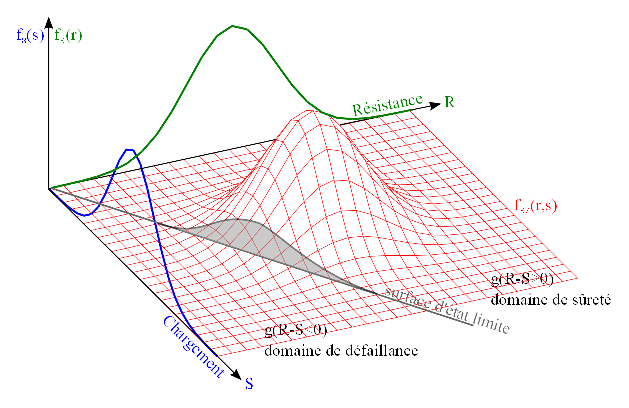
\includegraphics[width=110mm]{fiabilite.eps}
\caption{Illustration des concepts de fiabilité}\label{Fig-StoFiab}
\end{figure}

\medskip
En se plaçant dans l'espace de ces variables gaussiennes centrées réduites, dit \textcolorblue{espace réduit}, la fonction d'état limite représente toujours la limite entre les domaines de sûreté et de défaillance, mais de sorte que le point de cette hypersurface le plus proche de l'origine, appelé \textcolorblue{point de conception}, est le point pour lequel la probabilité de défaillance est maximale.
Cette distance à l'origine est appelée \textcolorblue{indice de sûreté~$\beta$}, et on a donc:
\begin{equation}\label{Eq-StoPf}
P_f = \Phi(-\beta)
\end{equation}
soit:
\begin{equation}
\beta = -\Phi^{-1}(P_f)
\end{equation}
où~$\Phi$ est la fonction de répartition gaussienne centrée réduite.
Toutefois, déterminer ce point (i.e. le minimum de la fonction d'état limite) n'est pas si facile. Tous les algorithmes d'optimisation convergent vers un minimum, mais aucun ne peut affirmer que ce minimum est global.

\begin{histoire}
Le tout premier essai dans l'utilisation des concepts statistiques pour la fiabilité des structures dans de 1926, par Max Mayer\index[aut]{Mayer (Max), ?, Allemand} dans \emph{Die Sicherheit der Bauwerke und ihre Berechnung nach Grenzkräften anstatt nach zulässigen Spannungen}. De nombreux progrès ont été faits par M. Prot (\emph{Note sur la notion de coefficient de sécurité}, 1936), W. Weibul\index[aut]{Weibull (Ernst Hjalmar Waloddi), 1887-1979, Suédois} (\emph{Investigations into strength of properties of brittle materials}, 1938, \emph{A statistical theory of strength of materials}, 1939), W. Kjellman\index[aut]{Kjellman (Walter), 1905-1955, Suédois} (\emph{Säkerhetproblemet ur principiell och teoretisk synpunkt}, 1940), et G. Wästlund\index[aut]{Wästlund (Karl Georg), 1905-1980, Suédois} (\emph{Säkerhetproblemet ur praktisk-konstruktiv synpunkt}, 1940), mais globalement, très peu d'articles avaient été publiés dans le domaine avant la seconde guerre mondiale.

\sbox{\MaBoiteAvecPhotos}{\setlength{\tabcolsep}{0pt}\scriptsize%
\begin{tabular}{cc}%
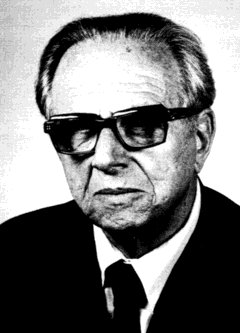
\includegraphics[height=\the\HauteurDesPhotos]{Freudenthal}&
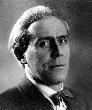
\includegraphics[height=\the\HauteurDesPhotos]{Gumbel}\\%
Freudenthal&Gumbel%
\end{tabular}}
\medskip\ifVersionDuDocEstVincent\else\vspace{\smallskipamount}\fi
\ImageADroite{%
Après 1945, le nombre d'article croit constamment. A l'université de Columbia, A.M.~Freudenthal\index[aut]{Freudenthal (Alfred Martin), 1906-1977, Américain} créa un institut pour l'étude de la fatigue et de la fiabilité, et produisit un grand nombre d'articles. L'évolution des codes modernes a été grandement influencée par les articles de 1949 à 1952 de E.~Torroja\index[aut]{Torroja (Eduardo), ?, Espagnol} et A.~P\'aez\index[aut]{P\'aez (A.), ?, Espagnol} (par exemple \emph{Calcul du coefficient de sécurité}, 1952).
En 1953, dans sa thèse \emph{Strength, safety and economical dimension of structures}, A.I.~Johnson\index[aut]{Johnson (A.I.), ?, Suédois}  suggéra d'utiliser les distributions de valeurs extrêmes, celles-ci étant étudiées par E.J.~Gumbel\index[aut]{Gumbel (Emil Julius), 1891-1966, Allemand} (\emph{Statistics of Extremes}, 1958).}

J.~Ferry Borges en 1952 pointa l'importance de prendre en compte le caractère aléatoire des dimensions et des propriétés mécaniques dans celui du comportement structurel. Dans un rapport établi en 1962 par A.M.~Freundenthal il est suggéré de représenter le chargement par une distribution en valeurs extrêmes et la résistance pour une distribution normale logarithmique.

\sbox{\MaBoiteAvecPhotos}{\setlength{\tabcolsep}{0pt}\scriptsize%
\begin{tabular}{cc}%
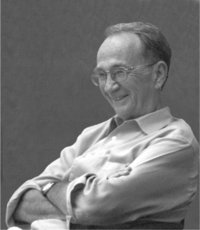
\includegraphics[height=\the\HauteurDesPhotos]{Cornell}&
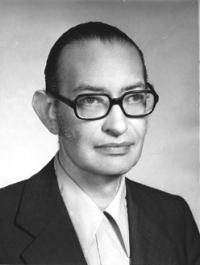
\includegraphics[height=\the\HauteurDesPhotos]{Rosenblueth}\\%
Cornell&Rosenblueth%
\end{tabular}}
\medskip\ifVersionDuDocEstVincent\else\vspace{\smallskipamount}\fi
\ImageAGauche{
En 1967, C.A.~Cornell\index[aut]{Cornell (Carl Allin), 1938-2007, Américain} dans deux articles (\emph{Bounds on the reliability of structural systems} et \emph{A probability-based structural code}) propose une représentation du chargement, de la résistance et des dimensions par leurs moyenne et variance, ce qui devient la base des méthodes dites de niveau II$\,^a$. %\footnotemark ou\footnotemark[1] ne fonctionnent pas ici (donne 1. et pas a. car environnement dans environnement
D'importantes contributions dans ce domaine seront dues à E.~Rosenblueth\index[aut]{Rosenblueth (Emilio), 1926-1994, Mexicain} et L.~Esteva\index[aut]{Esteva (Luis), 1935-2012, Mexicain} en 1972, O.~Ditlevsen\index[aut]{Ditlevsen (Ove Dalager), 1935-, Danois} en 1973, A.M.~Hasofer\index[aut]{Hasofer (A. M.),} et N.C.~Lind\index[aut]{Lind (Niels Christian),} en 1974 et D.~Veneziano en 1974. Nous allons en dire quelques mots un peu plus bas (indices de fiabilité).}

En 1968, dans un article sur la conception sous chargement sismique (\emph{Probabilistic models for seismic force design}) J.R.~Benjamin défend l'utilisation des concepts probabilistes Bayésiens.
%Toujours en 1968, A.H. Ang et M. Amin, dans \emph{Reliability of structures and structural systems}, proposent de diviser le facteur total en deux parties dans le but de diminuer la sensibilité du type de distribution.
Quant aux recherches des scientifiques russes sur le sujet, elles sont publiées par V.V.~Bolotin\index[aut]{Bolotin (Vladimir V.), 1926-?, Russe} en 1969 dans \emph{Statistical methods in structural mechanics}.

\sbox{\MaBoiteAvecPhotos}{\setlength{\tabcolsep}{0pt}\scriptsize%
\begin{tabular}{ccccc}%
%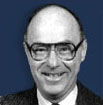
\includegraphics[height=\the\HauteurDesPhotos]{Moses}&
\includegraphics[height=\the\HauteurDesPhotos]{Rackwitz}&

\includegraphics[height=\the\HauteurDesPhotos]{Karadeniz}&
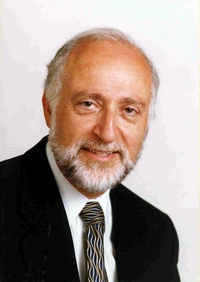
\includegraphics[height=\the\HauteurDesPhotos]{DerKiureghian}&
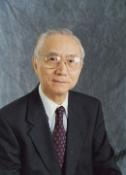
\includegraphics[height=\the\HauteurDesPhotos]{Shinozuka}&
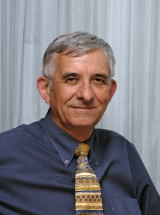
\includegraphics[height=\the\HauteurDesPhotos]{Lemaire}\\%
%Moses&
Rackwitz&Karadeniz&Der Kiureghian&Shinozuka&Lemaire%
\end{tabular}}
\medskip\ifVersionDuDocEstVincent\else\vspace{\smallskipamount}\fi
\ImageADroite{%
Depuis 1970, de très nombreux articles ont été publiés sur le sujet. N'en mentionner que quelque uns est faire offense à de nombreux très bons autres articles. Nous citerons encore quelques grands noms du domaine tels que J.~Armit (\emph{wind structures}, 1976), F.~Moses (\emph{Reliability of structural systems}, 1976),\index[aut]{Moses (Fred), ?-, Américain} R.~Rackwitz\index[aut]{Rackwitz (Rüdiger), 1941-2012, Allemand} (\emph{First order reliability theories and stichastic models}, 1977), H.~Karadeniz\index[aut]{Karadeniz (Halil), 1946-, Turque} (logiciel SAPOS), A.~Der Kiureghian\index[aut]{Der Kiureghian (Armen), 1947-, Arménien}, M.~Shinozuka\index[aut]{Shinozuka (Masanobu), 1930-, Japonais}, M.~Lemaire\index[aut]{Lemaire (Maurice), ?-, Français}...}
\footnotetext[1]{On distingue les méthodes de:
\begin{itemize}
   \item niveau I: l'aspect probabiliste est introduit en donnant aux variables aléatoires une «valeur caractéristique» associée à un facteur de sécurité partiel;
   \item niveau II: ce sont les méthodes fiabilistes utilisant deux paramètres pour décrire chaque variable aléatoire (moyenne et variance);
   \item niveau III: elles procèdent à l'analyse complète du problème et impliquent l'intégration de la fonction de densité de probabilité conjointe multidimensionnelle des variables aléatoires étendue sur le domaine de la sécurité. La fiabilité est exprimée en termes d'indices de sécurité adéquates, à savoir: indice de fiabilité et probabilité de défaillance;
   \item niveau IV: elles concernent les structures qui sont d'une importance économique majeure, et impliquent l'utilisation des principes de l'analyse économique de l'ingénierie sous incertitude. Elles tiennent compte des coûts et des bénéfices de la construction, de la maintenance, de la réparation, des conséquences de la défaillance, des intérêts sur le capital... Elles doivent être utilisées pour les projets sensibles comme les projets nucléaires, les tours de transmission, les ponts routiers.
\end{itemize}}

\medskip\ifVersionDuDocEstVincent\else\vspace{\medskipamount}\fi
Revenons un peu sur \textcolorblue{L'indice de fiabilité} utilisé en analyse de risque. C'est une mesure de la sûreté qui est élevé lorsque la probabilité de défaillance~$P_f$ est faible. Il s'agit d'un outil plus rudimentaire que la probabilité de défaillance qui est utilisé si celle-ci est trop grande ou lorsque son calcul est trop incertain à cause de l'approximation faite ou parce que l'on ne dispose pas d'informations suffisantes pour la calculer.

En 1969, Cornell\index[aut]{Cornell (Carl Allin), 1938-2007, Américain} définit l'indice de fiabilité~$\beta_c$ (dans le cas de variables gaussiennes) comme:
\begin{equation}
\beta_C=\dfrac{\E{M}}{D[M]}
\end{equation}
L'idée est que la distance du point de mesure~$\E{M}$ à la surface d'état limite est une bonne mesure de la fiabilité. Cette distance est mesurée par rapport à une unité d'incertitude~$D[M]$ qui peut être la variance par exemple. On appelle~$M$ la marge de sécurité.

Si l'on note~$r$ la résistance et~$s$ le chargement correspondant, alors~$g(r,s)=r-s$ et~$M=R-S$. On peut alors écrire:
$$\beta_C=\dfrac{\mu_R-\mu_S}{\sqrt{\sigma_R^2+\sigma_S^2}}$$

En 1972, Rosenblueth\index[aut]{Rosenblueth (Emilio), 1926-1994, Mexicain} et Esteva\index[aut]{Esteva (Luis), 1935-2012, Mexicain} proposent un nouvel indice de fiabilité. Dans le cas où~$R>0$ et~$S>0$, on peut écrire~$g(r,s)=\log(r/s)$, et~$M=\log(r/s)$, d'où:
\begin{equation}
\beta_{RE}=\dfrac{\E{\log(r/s)}}{D[\log(r/s)]}
\end{equation}
qui est calculé en linéarisant la marge de sécurité~$M$. Un développement de Taylor au premier ordre donne:
$$M\approx\dfrac{\log\mu_R-\log\mu_S}{\sqrt{\sigma_R^2+\sigma_S^2}}$$

En 1974, Hasofer\index[aut]{Hasofer (A. M.),} et Lind\index[aut]{Lind (Niels Christian),} proposent de passer de l'espace des variables~$X$ à celui de variables normalisées et non corrélées. Ce sont eux qui donnent la définition de l'indice de fiabilité~$\beta_{HL}$ comme la distance minimale de l'origine à la surface d'état limite.
En 1976, Ditlevsen\index[aut]{Ditlevsen (Ove Dalager), 1935-, Danois} propose un autre indice de fiabilité, plus sélectif, en introduisant une mesure de fiabilité obtenue en intégrant une fonction pondérée sur le domaine de sûreté. En pratique, on a souvent~$\beta_G=\beta_{HL}$.
\end{histoire}

\medskip
\subsection{Méthodes FORM/SORM}
La probabilité de défaillance~$P_f$ donnée à l'équation~(\ref{Eq-StoPf}) est rarement utilisable directement, le domaine d'intégration étant défini implicitement. La méthode \textcolorblue{FORM} (First Order Reliability Method) permet d'obtenir une approximation de cette intégrale.

On commence par réécrire l'équation~(\ref{Eq-StoPf}) dans l'espace réduit. Pour cela on utilise une transformation isoprobabiliste~$T : X \rightarrow U(X)$. Les transformations couramment utilisées sont celles de Rosenblatt\index[aut]{Rosenblatt (Murray), 1926-, Américain} ou Nataf\index[aut]{Nataf (André), ?, Français}\footnote{La transformation de Rosenblatt transforme un vecteur~$X$ de loi quelconque en un vecteur~$U$ de même dimension mais à composantes indépendantes, gaussiennes, centrées et réduites. La transformation de Nataf transforme un vecteur ayant une loi à copule elliptique en un vecteur de loi sphérique associée au représentant elliptique de la copule. Une copule est une fonction de répartition définie sur~$[0,1]^N$ dont les lois marginales sont égales à la loi uniforme sur~$[0,1]$. Nous nous passerons volontiers de cela dans ce document de présentation. Pour la petite histoire, Murray Rosenblatt a passé sa thèse sous la direction de Mark Kac.}. En utilisant ce changement de variable, on obtient:
\begin{equation}\label{Eq-StoPfU}
P_f=\dint_{T^{-1}(U),S(T^{-1}(U)))} \varphi_n(U) \dd u_1...\dd u_n
\end{equation}
avec~$\varphi_n$ la densité de probabilité multinormale de dimension~$n$:
\begin{equation}
\varphi_n(u)=\dfrac1{(\sqrt{2\pi})^n}\exp\PP{-\dfrac12(u_1^2+...+u_n^2)}
\end{equation}
Cette densité de probabilité est maximale à l'origine et décroît exponentiellement avec~$\|u\|^2$. Les points contribuant le plus à l'intégrale sont donc ceux appartenant au domaine de défaillance les plus proches de l'origine.

Puis on détermine le point de conception~$P$, i.e. le point~$D_f$ le plus proche de l'origine:
\begin{equation}
P = \min_{\|u\|} \left\{g(T^{-1}(U),S(T^{-1}(U)))\le0\right\}
\end{equation}
en utilisant un algorithme d'optimisation pour résoudre ce problème de minimisation.

Enfin on approche le domaine d'intégration~$D_f$ dans (\ref{Eq-StoPfU}) par le demi-espace défini par l'hyperplan tangent à~$D_f$ en~$P$. L'intégration est alors analytique, et on obtient l'équation~(\ref{Eq-StoPf}).

\medskip
Les méthodes \textcolorblue{SORM} (Second Order Reliability Method) sont des extensions de la méthode FORM.
L'une d'elle consiste à approcher la surface d'état limite par un hyperparaboloïde d'ordre 2 au voisinage du point de conception. Si~$(\kappa_1, ..., \kappa_{n-1})$ désignent les courbures principales de cet hyperparaboloïde, l'approximation SORM de la probabilité de défaillance conduit à la formule de Breitung:
\begin{equation}
P_f = \Phi(-\beta)\prod_{i=1}^{n-1}\dfrac1{\sqrt{1-\beta_{\kappa_i}}}
\end{equation}

\medskip
\subsection{Tirages d'importance}

Les simulations de Monte Carlo\index{méthode de Monte-Carlo} sont les méthodes les plus simples à mettre en œuvre pour calculer la probabilité de défaillance d'un système, mais ce sont aussi les plus coûteuses. Après avoir généré des réalisations pour les variables aléatoires d'entrée selon leur densité conjointe de probabilité, on évalue la fonction d'état limite pour ces réalisations. On compte le nombre total de cas défaillants parmi les calculs effectués, ce qui permet d'estimer la probabilité en fonction du nombre de cas défaillants par rapport au nombre total des réalisations effectuées. Pour s'assurer de la convergence des méthodes de simulation, il faut calculer le coefficient de variation de la simulation: la convergence est atteinte pour un coefficient de variation d'environ 5\%.

Les \textcolorblue{simulations d'importance} (ou Importance sampling) sont des méthodes efficaces pour estimer la probabilité de défaillance, car elles permettent de générer des tirages qui conduisent plus fréquemment à la défaillance et permettent d